\documentclass[letterpaper,11pt]{article}
\usepackage{graphicx}
\usepackage{listings}
\usepackage[super]{nth}
\usepackage[hyphens]{url}
\usepackage{hyperref}
\usepackage{amsmath}
\usepackage[makeroom]{cancel}
\usepackage[table]{xcolor}
\usepackage{comment}
\usepackage[space]{grffile}
\usepackage{csvsimple}

\newcommand*{\srcPath}{../src}%

\lstset{
	basicstyle=\footnotesize,
	breaklines=true,
}

\begin{document}

\begin{titlepage}

\begin{center}

\Huge{Assignment 8}

\Large{CS 532:  Introduction to Web Science}

\Large{Spring 2018}

\Large{Hrishi Gadkari}



\end{center}

\end{titlepage}

\newpage


% =================================
% First question
% =================================
\section*{1}


\subsection*{Question}

\begin{verbatim}
1. Create two datasets; the first called Testing, the second called Training. 
	
The Training dataset should:
a. consist of 10 text documents for email messages you consider 
spam (from your spam folder)
b. consist of 10 text documents for email messages you consider 
not spam (from your inbox)

The Testing dataset should:
a. consist of 10 text documents for email messages you consider 
spam (from your spam folder)
b. consist of 10 text documents for email messages you consider 
not spam (from your inbox)

Upload your datasets on github

\end{verbatim}
\clearpage
\subsection*{Answer}

For the above question, I went through my gmail spam folder which had enough spam emails to download. I downloaded 20 emails in pdf file format. As the emails had to be in text format, I converted them using \cite{pdftext}. I made two folders test and train in which I pasted 10 spam emails individually as spam(count).txt. I then downloaded 20 emails from the inbox of my same gmail account which I used for downloading spam emails. They were also in pdf format which I later converted into \cite{pdftext} and pasted into train and test folders containing 10 emails each as nonspam(count).txt. After this I uploaded them on my Github account\cite{gitref}.

\begin{figure}[h]
\centering
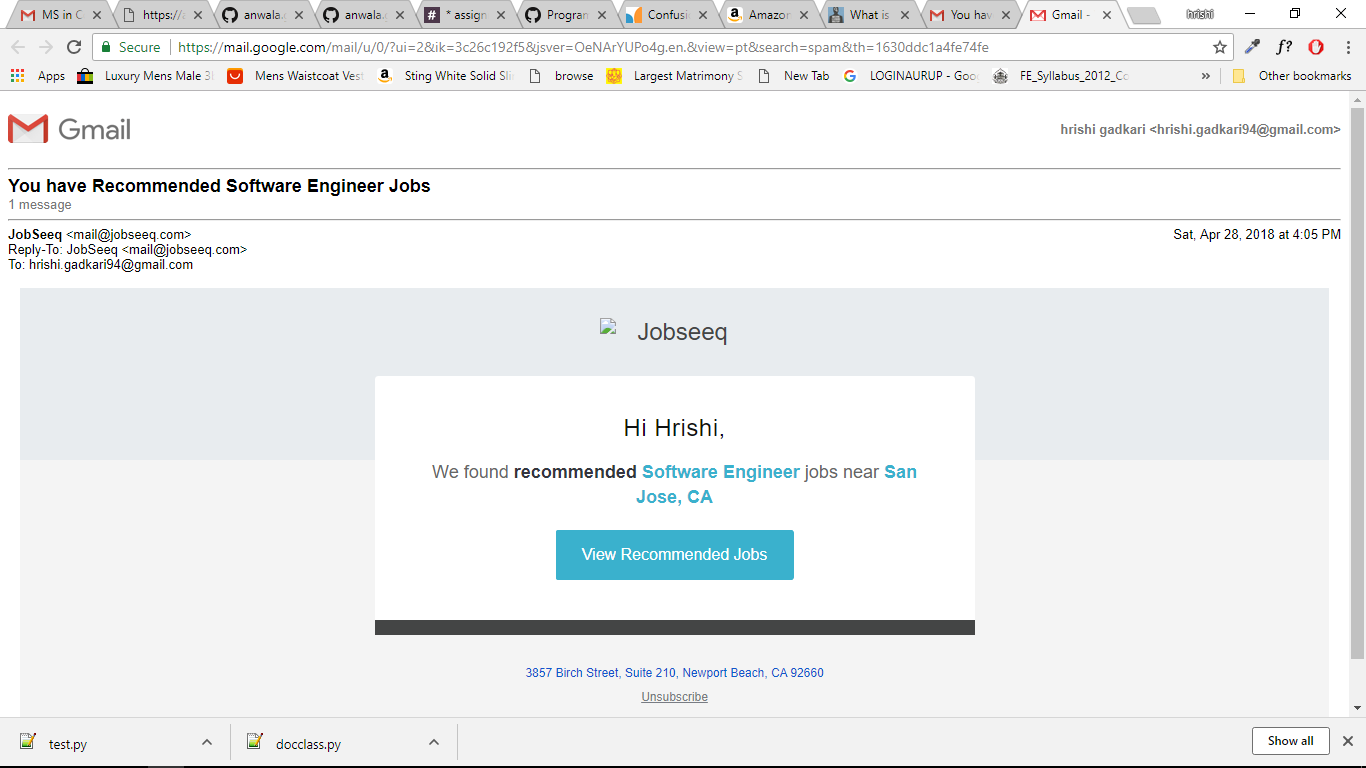
\includegraphics[scale=0.33]{pdf.png}
\caption{Emails downloaded in pdf format}
\label{fig:q1cali}
\end{figure}


\clearpage

% =================================
% Second question
% =================================

\section*{2}

\subsection*{Question}

\begin{verbatim}

2. Using the PCI book modified docclass.py code and
test.py (see Slack assignment-8 channel)
Use your Training dataset to train the Naive 
Bayes classifier ( e.g., docclass.spamTrain() )
Use your Testing dataset to test (test.py) the Naive 
Bayes classifier and report the classification results.

\end{verbatim}
 \clearpage
\subsection*{Answer}		

In order to train the Training dataset, I modified the \textbf{docclass.py} code as discussed in Slack assignment8 channel. The code is as follows:

\lstinputlisting[frame=single,caption={Python program to train the dataset with Naive Bayes Classifier},label=lst:q2query,captionpos=b,numbers=left,showspaces=false,showstringspaces=false,basicstyle=\footnotesize]{docclass.py}

The files read as spam for training, I passed \textbf{spam} as a classifier in the second argument of the \textbf{c1.train} function whereas file read as nonspam , I passed \textbf{not spam}. The code is written in a function called \textbf{eTrain()}
I then modified the \textbf{test.py} to test the Naïve Bayes classifier on the Testing dataset as follows.

\lstinputlisting[frame=single,caption={Python program to test the dataset with Naive Bayes Classifier},label=lst:q2tfidf,captionpos=b,numbers=left,showspaces=false,showstringspaces=false,basicstyle=\footnotesize]{test.py}


\begin{figure}[h]
\centering
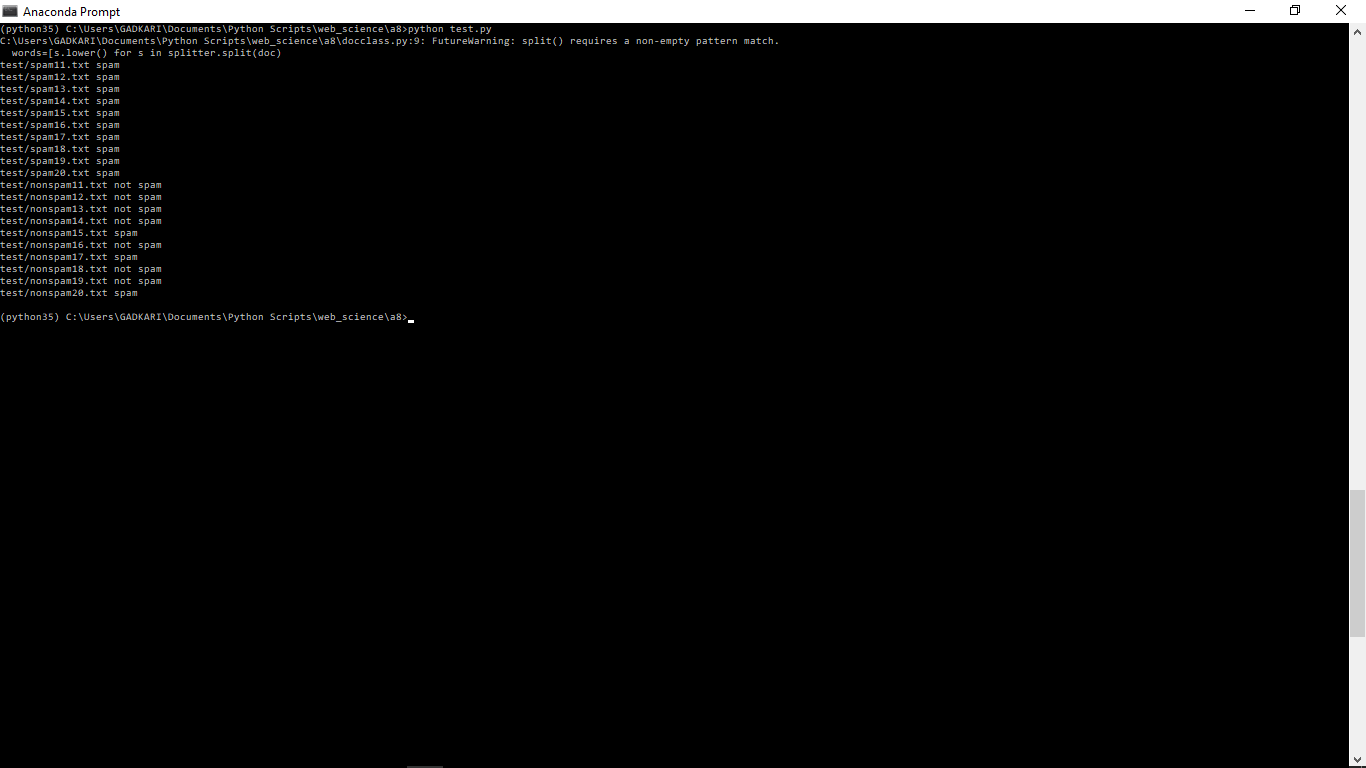
\includegraphics[scale=0.33]{classification.png}
\caption{Classification Results }
\label{fig:q2naive}
\end{figure}

From the result we could see it identified 10/10 spam files as spam and 7/10 as non-spam. I think it did a  good job. 


\clearpage


\section*{3}

\subsection*{Question}

\begin{verbatim}
==================================
===Each question below is for 3 points extra credit===
==================================

3. Draw a confusion matrix for your classification results
(see: https://en.wikipedia.org/wiki/Confusion_matrix)

\end{verbatim}

\clearpage
\subsection*{Answer}

In-order to understand a confusion matrix I went through \cite{conref} as mentioned in the question. As per the classification results and by the understanding of confusion matrix, the matrix would look as above:


\begin{table}
\begin{tabular}{ | l | l | p{8.2cm} | }
\hline
\textbf{Confusion Matrix} & \textbf{Predicted Spam} & \textbf{Predicted Non Spam} \\
\hline
\textbf{True Spam} & 10  & 0 \\
\hline
\textbf{True Non Spam} & 3 & 7 \\
\hline
\end{tabular}
\caption{Confusion Matrix}
\label{table:conf}
\end{table}

\clearpage


\section*{4}

\subsection*{Question}

\begin{verbatim}

4. Report the precision and accuracy scores of your classification results
(see: https://en.wikipedia.org/wiki/Precision_and_recall)

\end{verbatim}

\clearpage
\subsection*{Answer}

.For calculating precision I went through the \cite{precref} as mentioned in the question. Based on the classification results the precision is calculated as follows:

\begin{verbatim}

precision =         true positives                      =       10        =  1
                  ---------------------------------------    -----------
                      true positives + false positives       10 + 0

\end{verbatim}

For calculating the accuracy score I went through \cite{accref} and calculated as follows:

\begin{verbatim}

accuracy =    correct predictions      =        10 + 7          =  0.85
              -------------------------       -------------------
                      total predicyions          10 + 0 + 3 + 7

\end{verbatim}


\clearpage


% =================================
% Bibliography
% =================================

\begin{thebibliography}{9}
\bibitem{pdftext}
``Convert PDF to Text Online'' PDF to Text, n.d. Web. April 30, 2018. \url{http://pdftotext.com/}.
\bibitem{gitref}
``GitHub.''Hrishi29/anwala.github.io.,n.d. Web. April 30, 2018. \url{https://github.com/Hrishi29/anwala.github.io/tree/master/Assignments}
\bibitem{conref}
``Confusion matrix.'' Wikipedia, April 27, 2018. Web. April 30, 2018. \url{https://en.wikipedia.org/wiki/Confusion_matrix}
\bibitem{precref}
``Precision and recall.''   Wikipedia, April 09, 2018. Web. April 30, 2018. \url{https://en.wikipedia.org/wiki/Precision_and_recall}
\bibitem{accref}
What is a Confusion Matrix in Machine Learning ``Machine Learning Mastery .'' December 05, 2017. N.p., Web. April 30, 2018. \url{https://machinelearningmastery.com/confusion-matrix-machine-learning/}

\end{thebibliography}

\end{document}